\documentclass[oneside, a4paper, 11pt]{report}

\usepackage{ngerman}
\usepackage{graphicx}
\usepackage{xcolor}
\usepackage[T1]{fontenc}
\usepackage[latin1]{inputenc}
\usepackage{lmodern}
\usepackage{geometry}
\usepackage[numbers]{natbib}
\usepackage[pagestyles]{titlesec}
\usepackage{titletoc}
\usepackage{microtype}
\usepackage{booktabs}
\usepackage{caption}
\usepackage{subcaption}
\usepackage{setspace}
\usepackage{calc}
\usepackage[colorlinks]{hyperref}
\usepackage{amsmath,amsfonts,amssymb,amsthm}
\usepackage{mathtools}
\usepackage[version=3]{mhchem}
\usepackage{wrapfig}
\usepackage{tikz}
\usepackage{cancel}
\usepackage{algorithm}
\usepackage{algpseudocode}
\usepackage{wasysym}
\usepackage{array}
\usepackage{listings}

\renewcommand\abstractname{Vorwort}

% Layout der "Uberschriften
\titleformat{\chapter}[hang]
{\fontfamily{pag}\Large\bfseries}{\thechapter}{1.5cm-\widthof{\thechapter}}{\large}
\titleformat{\section}
{\fontfamily{pag}\normalsize\bfseries}{\thesection}{1.5cm-\widthof{\thesection}}{\normalsize}
\titleformat{\subsection}
{\fontfamily{pag}\normalsize\bfseries}{\thesubsection}{1.5cm-\widthof{\thesubsection}}{\normalsize} 


\newpagestyle{mystyle}
{
	\headrule
	\sethead{\thechapter. \chaptertitle}{}{\thepage}
	%
	\footrule
	\setfoot{\textnormal{Datenbank}}\raggedleft{\textnormal{Jascha Petter}}
} 
\pagestyle{mystyle}
\parindent0pt
\onehalfspacing
\geometry{outer=20mm,  inner=25mm,  top=20mm,  bottom=30mm}
%
\author{Jascha Petter}
%
\begin{document}
	\begin{titlepage}
		\begin{center}
			
\includegraphics[width=0.4\linewidth]{image2.jpg}\\
			\vspace*{3.5cm}
			\Huge{\bf Quadrocopter Raspberry Pi 2016\bigskip\bigskip\\}
			\LARGE{Datenbank mit PythonMySQL\bigskip\bigskip\\}
			\large{Universit"at T�bingen\vfill}
		\end{center}
		%
		\vspace*{1cm}
		\begin{minipage}{\widthof{Jascha Petter}}
			\begin{flushleft}
				Author:\\
				Jascha Petter
			\end{flushleft}
		\end{minipage}
		\hfill
		\begin{minipage}{\widthof{\today}}
			\begin{flushright}
				Dienstag 20.08.16
			\end{flushright}
		\end{minipage}
	\end{titlepage}
	\begin{abstract}	
		Hier k"onnte ihr Vorwort stehen
	\end{abstract}
	%Inhalts- und Abbildungsverzeichnis
	\newpage
	\pagenumbering{Roman}
	\begingroup
	\let\clearpage\relax
	\tableofcontents
	\listoffigures
	\endgroup
	\newpage
	\pagenumbering{arabic}
	%
	\chapter{Einrichtung}
		\section{MySQL}
			\begin{enumerate}
				\item[] 
					Um auf ihrem System einen MySQL Server laufen zu lassen, ben"otigen Sie den \glqq{}MySQL Community Server\grqq{}.
				\item 
					Laden Sie sich hierzu den MySQL Community Server von der MySQL Homepage herunter.
						\begin{center}
							\url{http://dev.mysql.com/downloads/mysql/}\footnote{stand 20.09.2016}
						\end{center}
					W"ahlen Sie dort die dementsprechende Version f"ur Ihr System. Sie m"ussen sich f"ur den Download nicht anmelden, oder ein Konto erstellen. Klicken Sie einfach auf \glqq{}No thanks, just start my download\grqq{}. 
				\item
					Nach der Installation wir Ihnen das Passwort f"ur den Root User angezeigt.
					\begin{figure}[h!]
						\centering
						\includegraphics[width=0.4\linewidth]{rootPW.png}
						\caption{Passwort Alert \label{pw_alrt}}
					\end{figure}\\
					Notieren Sie sich dieses, da es sp"ater noch gebraucht wird!
				\item 
					"Offen sie nun Ihren Termial und geben folgende Befehle ein, um ein neues Passwort zu vergeben:
					\begin{verbatim}
						$ cd /usr/local/mysql/bin
						$ ./mysqladmin -u root -p password '<password>'
					\end{verbatim}
					Sie werden nun aufgefordert ihr Root Passwort, welches Sie vorhin notiert haben, einzugeben.
					\begin{verbatim}
						$ exit
					\end{verbatim}
					Um zur"uckzukehren
				\newpage
				\item
					Nun erstellen wir einen neuen Benutzer und geben diesem die Notwendigen Rechte.
					\begin{verbatim}
					$ ./mysql -u root -p
					mysql > CREATE USER 'PiSense'@'localhost' IDENTIFIED BY 'somePW';
					mysql > GRANT ALL PRIVILEGES ON *.* TO 'PiSense'@'localhost';
					\end{verbatim}
					Dies ist nun der neue Benutzer, mit dem gearbeitet wird.
				\item
					Nun muss noch der MySQL-Server gestartet werden. Dies ist wie folgt m"oglich.
					\begin{verbatim}
						$ cd /usr/local/mysql/support-files/
						$ sudo ./mysql.server  start
					\end{verbatim}
			\end{enumerate}
		\section{Datenbank}
			\begin{enumerate}
				\item[]
					Da wir nun einen Benutzer zum arbeiten habe, fehlt nur noch die Datenbank und eine Tabelle. 
				\item 
					Zu erst muss ein neues Schema erstellt werden:
					\begin{verbatim}
						CREATE DATABASE `SenseData` COLLATE 'latin1_swedish_ci';
					\end{verbatim}
				\item
					Nun k"onnen wird eine Tabelle anlegen:
					\begin{verbatim}
						CREATE TABLE `SenseData`.`DATA` (
						`PITIME` timestamp(2) PRIMARY KEY NOT NULL,
						`ACC_X` double NOT NULL,
						`ACC_Y` double NOT NULL,
						`ACC_Z` double NOT NULL,
						`MAG_X` double NOT NULL,
						`MAG_Y` double NOT NULL,
						`MAG_Z` double NOT NULL,
						`G_ROLL` double NOT NULL,
						`G_PITCH` double NOT NULL,
						`G_YAW` double NOT NULL,
						`TEMP` double NOT NULL,
						`PRESS` double NOT NULL,
						`M1` double NOT NULL,
						`M2` double NOT NULL,
						`M3` double NOT NULL,
						`M4` double NOT NULL
						) ENGINE='InnoDB' COLLATE 'latin1_swedish_ci';
					\end{verbatim}
					Zu den jeweiligen Eintr"agen sp"ater mehr.
			\end{enumerate}
			Somit ist die Datenbank vollst"andig erstellt und kann mit Daten gef"ullt werden.
		\newpage
		\section{Python}
			\begin{enumerate}
				\item[] 
					Um sp"ater Daten empfangen zu k"onne um diese in der Datenbank abzulegen ben"otigen wir Python. Da es sich um eine Skriptsprache handelt, ist eine IDE nicht vonn"oten. 
				\item
					Laden sie sich hierzu Python 2.7 von der Python Homepage herunter.
					\begin{center}
						\url{https://www.python.org/downloads/}\footnote{stand 20.09.2016}
					\end{center}
					Nach der Installation, k"onnen sie "uberpr"ufen ob es sich um die richtige version handelt mit:
					\begin{verbatim}
						$ python --version
					\end{verbatim}
				\item
					Damit Sie mit MySQL unter Python verwenden k"onnen, ben"otigen Sie noch MySQL-Python.
					\begin{center}
						\url{https://pypi.python.org/pypi/MySQL-python/}\footnote{stand 20.09.2016}
					\end{center}
			\end{enumerate}
			Nun ist alles komplett und Sie k"onnen beginnen.
	\chapter{Anwendung}
		Aufgabe des Python Skriptes ist es die Daten, welche vom Quadrocopter gemessen und per UDP versendet werden, entgegenzunehmen und in einer Datenbank abzulegen. Hierbei stellt das Skript eine Verbindung zu der Datenbank her und legt dort per INSERTs die empfangenen Daten ab.
		\section{Struktur der Datenbank}
			\begin{figure}[h!]
				\centering
				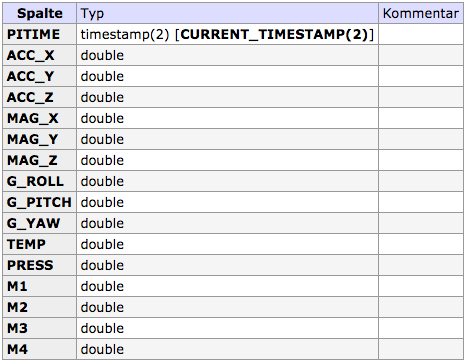
\includegraphics[width=0.4\linewidth]{tblstr.png}
				\caption{Struktur der Datenbank \label{db_str}}
			\end{figure}
			\begin{itemize}
				\item \underline{\textbf{PITIME}}\\
					PITIME ist die Zeit, welche momentan auf dem Pi herscht. Sie wurde als Primary Key gew"ahlt, da es zu jeder Zeit nur einen Messwert geben kann. Angegeben wird sie als Timestamp mit einen Genauigkeit von 10ms.
				\item ACC\_X/Y/Z\\
					Es werden alle drei Beschleunigungsachsen gespeichert, das Vorzeichen stellt hierbei die Richtung dar. 
				\item MAG\_X/Y/Z\\
					F"ur das Magnetfeld werden ebenfalls 3 Datens"azte abgelegt. 
				\item TEMP/PRESS\\
					Die Temperatur und der Luftdruck 
				\item M1/2/3/4
					F"ur die jeweiligen Motoren werden vier Datens"atze abgelegt, da diese sich unabh"anging von einander drehen k"onnen.
			\end{itemize}
		\newpage
		\section{Auszug aus der Datenbank}
			Hier ist ein beispielhafter Auszug der Datenbank zu sehen, er zeigt einen Ausschnitt aus der Demo.
			\begin{figure}[h!]
				\centering
				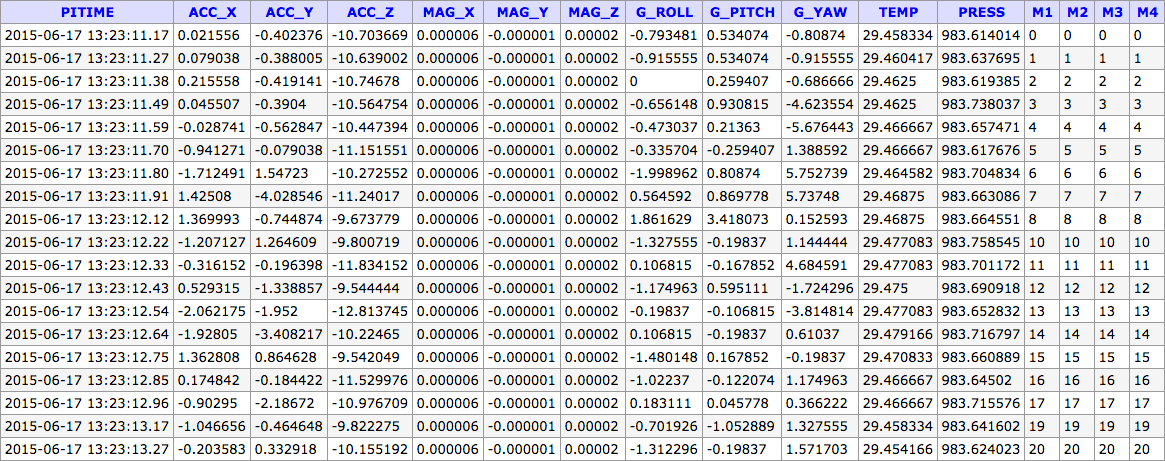
\includegraphics[width=0.9\linewidth]{bsptbl.png}
				\caption{Daten der Demo\label{demo_data}}
			\end{figure} 
		\section{Python}
			\subsection{Verbindung zur Datenbank}
				Um auf die vorhin erstelle Datenbank zuzugreifen, muss eine Verbindung hergestellt werden. Hierzu wird der neue Benutzer PiSense ben"otigt, nat"urlich k"onnten man auch Root benutzen das ist aber nicht Sinn der Sache.
				\begin{figure}[h!]
					\centering
					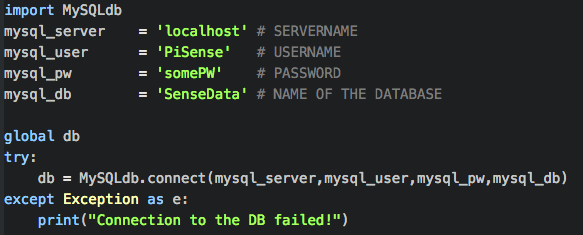
\includegraphics[width=0.65\linewidth]{dbc.png}
					\caption{Connector\label{dbc}}
				\end{figure}
			\newpage
			\subsection{UDP Socket}
				Damit das Skipt eine Message vom Quadrocopter empfangen kann, muss ein UDP Socket auf einem bestimmten Port Lauschen. Python stellt uns hierbei einen Receive-Funktion zur verf"ugung. Es muss nur die IP und der Port and einen Socket gebindet werden. 
				\begin{figure}[h!]
					\centering
					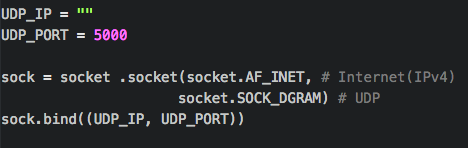
\includegraphics[width=0.65\linewidth]{udpsock.png}
					\caption{UDP Socket\label{UDPS}}
				\end{figure}\\
				In diesem Fall lauschen wir auf dem Port 5000, benutzen IPv4 und nat"urlich UDP.
			\subsection{Empfangen und aufteilen der Daten}
				\begin{figure}[h!]
					\centering
					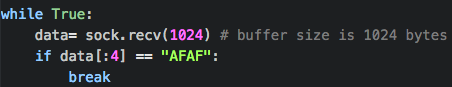
\includegraphics[width=0.65\linewidth]{whilerec.png}
					\caption{Empfange der Message\label{recv}}
				\end{figure}
				Es wird so lange gewartet bis eine Message ankommt, falls diese der String "AFAF" ist, wird das Skript beendet. Da die Daten in einem einzigen String ankommen, m"ussen sie herausgefiltert werden. Um dies zu erreichen wird der String bei jedem Zeilenumbruch getrennt. Nun m"ussen noch die Bezeichner \textit{abgeschnitten} werden. Auch hier liefert uns Python einen L"osung mit. Es werden die Vier ersten Zeichen verworfen.
				\begin{figure}[h!]
					\centering
					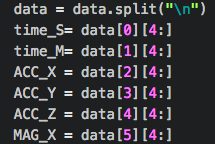
\includegraphics[width=0.3\linewidth]{trenn.png}
					\caption{Trennen der Daten\label{trenn_D}}
				\end{figure}
			\newpage
			\subsection{Ablegen der Daten}
				Damit die empfangenen Date jetzt nicht verloren gehen, werden sie in die Datenbank geschrieben. Dies erfolgt "uber einen INSERT. Hierbei werden die Daten in ihre jeweiligen Spalten der Tabelle gespeichert. Am ende muss das Query noch commited werden an die Datenbank.
				\begin{figure}[h!]
					\centering
					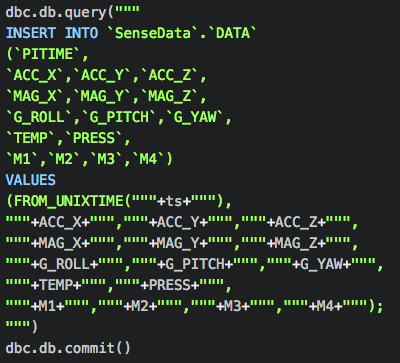
\includegraphics[width=0.5\linewidth]{query.png}
					\caption{Query\label{qry}}
				\end{figure}\\	
				Um sicherzustellen, dass das Skript funktioniert kann mit dem udpSend Skipt ein Senden des Quadrocopters simuliert werden. Jedoch handelt es sich hierbei nur um Zufallswerte. 
\end{document}
